\label{chap:polly}

This chapter explain the internals of  Polly - Polyhedral optimization
in llvm. The work is published in the First International workshop on PolyhedrAl Compilation
Techniques - IMPACT 2011\cite{pollypaper}.

\section{Introduction}

Today, effective polyhedral techniques exist to optimize computation intensive
programs.  Advanced data-locality optimizations are available to accelerate
sequential programs \cite{uday08pldi}. Effective methods to expose SIMD and
thread-level parallelism were developed and are used to offload calculations to
accelerators \cite{Baskaran10, Baghdadi_puttingautomatic}.  Polyhedral
techniques are even used to synthesize high-performance hardware
\cite{RISSET:2008}.

Yet, the use of programming-language-specific techniques significantly limits
their impact.  Most polyhedral tools use a basic, language specific front end
to extract relevant code regions. This often requires the source code to be in
a canonical form, disallowing any pointer arithmetic or higher level
language constructs like C++ iterators and prevents the optimization of
programs written in languages like Java or Haskell. Nevertheless, even tools
that limit themselves to a restricted subset of C may apply incorrect
transformations, as the effects of implicit type casts, integer wrapping or
aliasing are mostly ignored. To ensure correctness manual annotation
of code that is regarded safe to optimize is often required.  This prevents
automatic transformations and consequently reduces the impact of existing
tools.

In addition, significant optimization opportunities are missed by targeting a
programming language like C and subsequently passing it to a compiler. 
Effective interaction between polyhedral tools and
compiler internal optimizations are prevented. The only possible
way to pass information are source code annotations like C pragmas. As influencing
performance related decisions of the compiler is difficult, the resulting
program often suffers from poor register allocation, missed SIMDization or
similar problems.

With Polly we are developing a state-of-the-art polyhedral infrastructure for
LLVM, that supports fully automatic transformation of existing programs. Polly
detects and extracts relevant code regions without any human interaction. Since
Polly accepts LLVM-IR as input, it is programming language independent and
transparently supports constructs like C++ iterators, pointer arithmetic or
goto based loops. It is built around an advanced polyhedral library with full
support for existentially quantified variables and includes a state-of-the-art
dependency analysis. Due to a simple file interface it is easily possible to
apply transformations manually or to use an external optimizer. We use this
interface to integrate Pluto \cite{uday08pldi}, a modern data locality
optimizer and parallelizer. Thanks to integrated SIMD and OpenMP code
generation, Polly automatically takes advantage of existing and newly exposed
parallelism.

This chapter focuses on concepts of Polly which are new or little discussed in the polyhedral community.

\begin{figure}
  \label{fig:arch}
  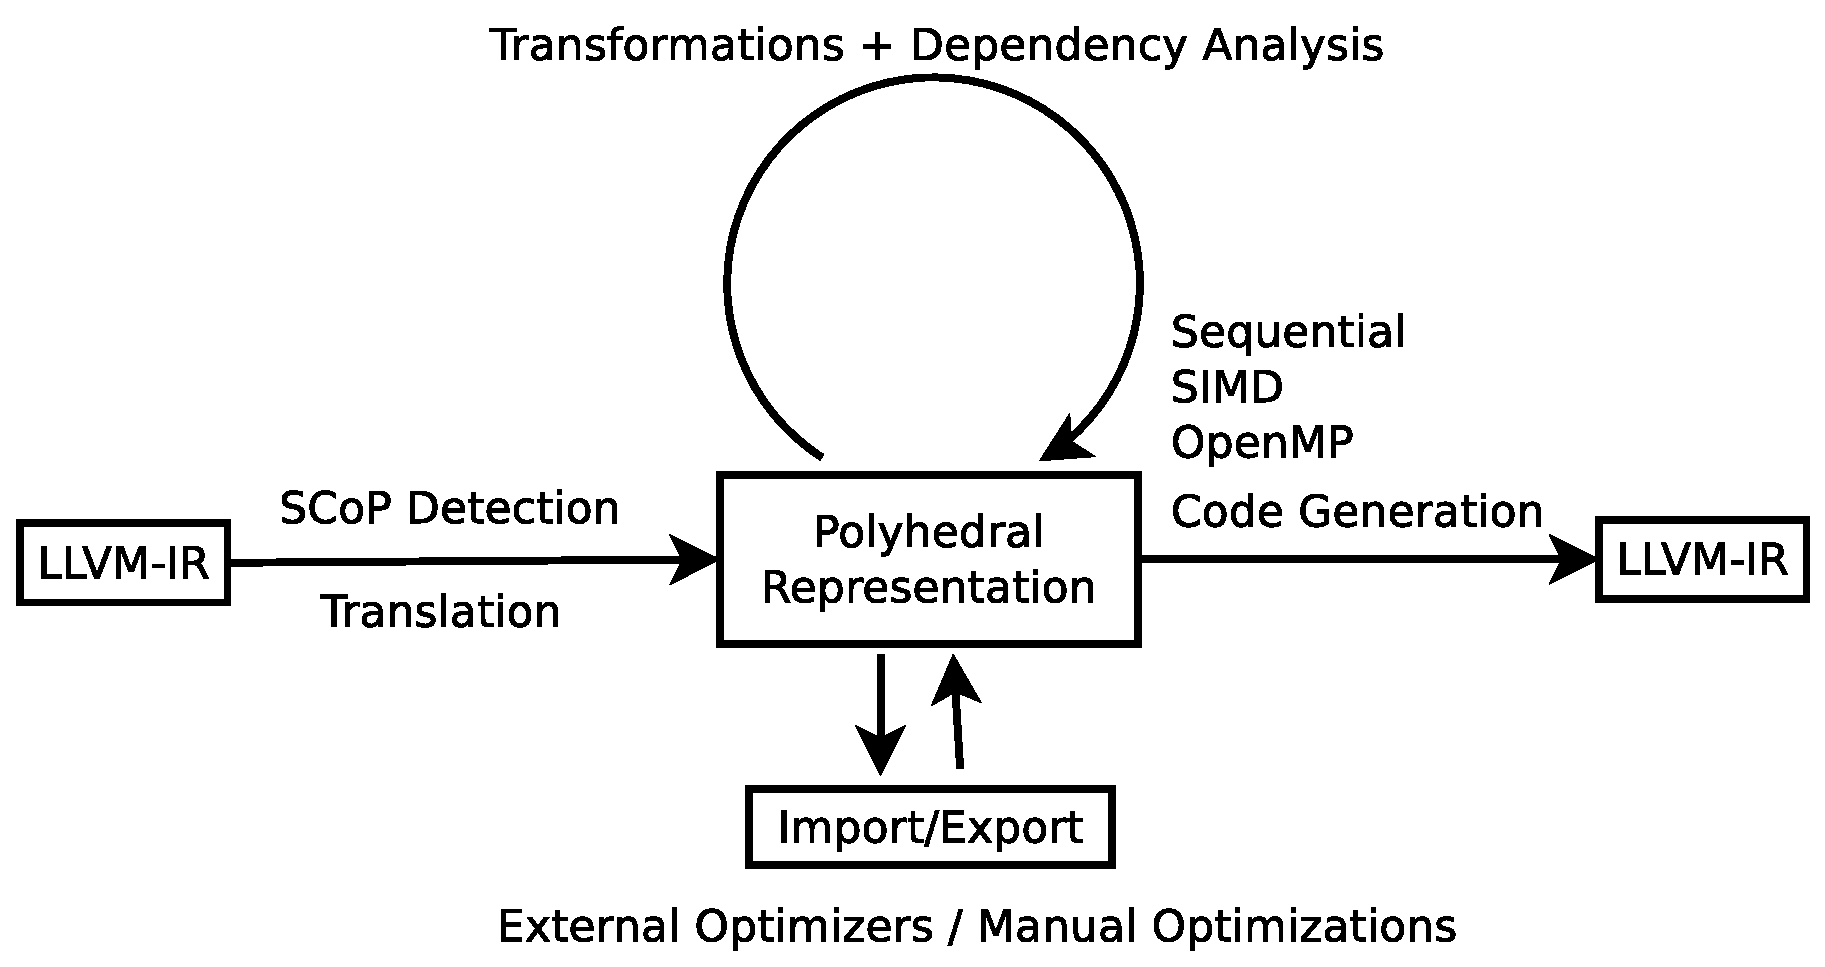
\includegraphics[width=1\textwidth]{images/architecture.eps}
  \caption{Architecture of Polly}
\end{figure}

\section{Implementation}

Polly is designed as a set of compiler internal analysis and optimization
passes. They can be divided into front end, middle end and back end passes. The
front end translates from LLVM-IR into a polyhedral representation, the middle
end transforms and optimizes this representation and the back end translates it
back to LLVM-IR. In addition, there exist preparing passes to increase the
amount of analyzable code as well as passes to export and reimport the polyhedral
representation.  Figure~\ref{fig:arch} illustrates the overall
architecture.

To optimize a program manually three steps are performed. First of all the
program is translated to LLVM-IR. Afterwards Polly is called to optimize LLVM-IR and
target code is generated. The LLVM-IR representation of a program can
be obtained from language-specific LLVM based compilers. clang is a
good choice for C/C++/Objective-C, DragonEgg for FORTRAN and ADA, OpenJDP or
VMKit for Java VM based languages, unladen-swallow for Python and GHC for
Haskell. Polly also provides a drop in replacement for \texttt{gcc} that is
called \texttt{pollycc}.

\subsection{LLVM-IR to Polyhedral Model}

To apply polyhedral optimizations on a program, the first step that needs to be
taken is to find relevant code sections and create a polyhedral description for
them. The code sections that will be optimized by Polly are static
control parts (SCoPs), the classical domain of polyhedral optimizations.
Extending the polyhedral model and therefore Polly to more general programs is
possible as shown by Benabderrahmane \cite{benabderrahmane.10.cc}.

\subsubsection{Region-based SCoP detection}
Polly implements a structured, region-based approach to detect
the SCoPs available in a function. It uses a refined version of the program
structure tree described by Johnson \cite{Johnson}.

A \emph{region} is a subgraph of the control flow graph (CFG) that is connected to the
remaining graph by only two edges, an entry edge and an exit edge.  Viewed as a
unit it does not change control flow. Hence, it can be modeled as a
simple function call, which can easily be replaced with a call to an optimized
version of the function.  A \emph{canonical region} is a region that cannot be
constructed by merging two adjacent smaller regions. A region \emph{contains}
another region if the nodes of one region are a subset of the nodes of the other
region. A tree is called \emph{region tree}, if the nodes of it are canonical regions
and the edges are defined by the contains relation.

To find the SCoPs in a function we look for the maximal regions that are valid
SCoPs. Starting from the outermost region, we look for canonical regions in the
region tree that are valid SCoPs. In case the outermost region is a valid SCoP,
we store it. Otherwise, we check each child. After analyzing the tree, we have a
set of maximal canonical regions that form valid SCoPs. These regions are now
combined to larger non-canonical regions such that, finally, the maximal 
non-canonical regions that form valid SCoPs are found.

\subsubsection{Semantic SCoPs}

In contrast to prevalent approaches based on the abstract syntax
tree (AST), Polly does not require a SCoP to match any specific syntactic
structure. Instead, it analyzes the semantics of a SCoP. We call SCoPs
that are detected based on semantic criteria \emph{semantic SCoPs}.

A common approach to detect a SCoP is to analyze an AST representation of
the program, that is close to the programming language it is implemented in. In
this AST control flow structures like for loops and conditions are
detected. Then it is checked if they form a SCoP. Common restrictions that need
to be met are the following. There exists a single induction variable for a
loop that is incremented from a lower bound to an upper bound by a stride of
one. Upper and lower bounds need to be expressions that are affine in parameters
and surrounding loop induction variables, where a parameter is any integer
variable that is not modified inside the SCoP.  The only valid statements are
assignments that store the result of an expression to an array element. The
expression itself uses side effect free operators with induction variables,
parameters or array elements as operands.  Array subscripts are affine
expressions in induction variables and parameters. There are various ways to
extend this definition of a SCoP, which we did not include in this basic
definition.

\begin{figure}

\begin{lstlisting}
                 for (i = 0; i < n + m; i++)
                       A[i] = i;
\end{lstlisting}
	\caption{A valid syntactic SCoP. Not always a valid semantic SCoP}
	\label{fig:syntacticScop}
\end{figure}

The detection of SCoPs as shown in Figure~\ref{fig:syntacticScop} with an AST
based approach is easily possible, however as soon as programs become more
complex and less canonical difficulties arise. The AST of a modern language is
often very expressive, such that there exist numerous ways a program can be
represented.  Sometimes different representations can be canonicalized.
However, as soon as goto based loops should be detected, various induction
variables exist or expressions are spread all over the program, sophisticated
analyses are required to check if a program section is a SCoP. Further
difficulties arise through the large amount of implicit knowledge that is
needed to understand a programming language.  A simple, often overlooked problem is integer
wrapping.  Assuming \texttt{n} and \texttt{m} are unsigned integers of 32 bit
width, it is possible that $n+m$~<~$n$ holds, because of the wrapping semantics
of C integer arithmetic \cite{c99}. The upper bound in the source code must
therefore be represented as $n+m\bmod 2^{32}$, but no polyhedral tool we know
of models the loop bound in this way. Further problems can be caused by
preprocessor macros, aliasing or C++ (operator) overloading. We believe even
standard C99 is too complex to effectively detect SCoPs in it. Tools like PoCC,
evade this problem by requiring valid SCoPs to be explicitly annotated in the
source code. However, this prevents any automatic optimization and
significantly limits the impact of polyhedral techniques.

Fortunately, after lowering programs to LLVM-IR the complexity is highly
reduced and constructs like implicit type casts become explicit. Furthermore,
it is possible to run a set of LLVM optimization passes, that further
canonicalize the code.  As a result, an
analysis that detects SCoPs based on their semantics is possible.  LLVM-IR is a
very low-level representation of a program, which does not have loops, but
jumps and gotos and has no arrays or affine expressions, but pointer arithmetic
and three address form operations. From this representation all necessary
information is recomputed using advanced compiler internal analyses available
in LLVM. Simple analyses used are loop detection or dominance information to
verify a SCoP contains only structured control flow. More sophisticated ones
check for aliasing or provide information about side effects of
function calls. 

An especially important aspect is how expressions for the loop bounds,
conditions or array subscripts are recovered. On LLVM-IR these expressions are
split into individual operations. Optimizations that transform multiplications into
shifts or a sequence of additions are very common. As a result, understanding
the effects of calculations on LLVM-IR is difficult.  Fortunately, LLVM
provides an analysis called scalar evolution \cite{Engelen01}, which calculates
closed form expressions for all scalar integer variables in a program.  It
abstracts away all intermediate calculations including calculations that
accumulate values over several loop iterations and describes the value of each
scalar as a chain of recurrence. The chain of recurrence
depends only on variables with values unknown at compile time and variables
describing the loop iteration at which it should be evaluated. As chains of
recurrence are more expressive than affine expressions, the work left for Polly
is to check if a chain of recurrence describes an affine expression and, if
this is the case, translate it into the corresponding affine expression. This
recovered affine expression can then be used to represent loop bounds, for
example.  The same concept is used to recover array accesses from plain memory
loads and stores, because address arithmetic is integer arithmetic.

As Polly successfully recovers all necessary information from a low-level
representation, there are no restrictions on the syntactic structure of the
program source code. A code section is accepted as soon as the LLVM analyses
can prove that it has the semantics of a SCoP. As a result, 
arbitrary control
flow structures are valid if they can be written as a well-structured set
of for-loops and if-conditions with affine expressions in lower and upper
bounds and in the operands of the comparisons. Furthermore, any set of
memory accesses is allowed as long as they behave like array accesses with affine subscripts.
A loop written
with \texttt{do..while} instead of \texttt{for} or fancy pointer arithmetic can easily be part of a valid SCoP.
To illustrate this we show two examples of valid SCoPs in Figure~\ref{semscop}.

\begin{figure}
\begin{verbatim}

// scop_one
  i = 0;
  
  do {
      int b = 2 * i;
      int c = b * 3 + 5 * i;
      A[c] = i;
      i += 2;
  } while (i < N);
\end{verbatim}

\begin{verbatim}
// scop_two
  int A[1024];
  
  void pointer_loop () {
      int *B = A;
      while (B < &A[1024]) {
          *B = 1;
          ++B;
      }
  }
\end{verbatim}
\caption{Valid semantic SCoPs}
\label{semscop}
\end{figure}

\subsection{Polyhedral Model}

\subsubsection{The integer set library} Polly uses isl, an integer set library
developed by Verdoolaege \cite{Verdoolaege10}. Isl natively supports
existentially quantified variables in all its data structures; therefore, Polly
also supports them throughout the whole transformation. This enables Polly to
use accurate operations on $\mathbb{Z}$-polyhedra instead of using polyhedra
in the rationals as approximations of integer sets.
Native support of $\mathbb{Z}$-polyhedra
simplified many internal calculations and we
expect it to be especially useful to represent the modulo semantics of integer
wrapping and type casts.


\subsubsection{Composable polyhedral transformations}
Polly uses the classical polyhedral description \cite{girbal}
that describes a SCoP as a
set of statements each defined by a domain, a schedule and a set of memory
accesses. The domain of a statement is the set of values the induction
variables surrounding the statement enumerate. For example, the statement in
Figure~\ref{fig:syntacticScop} has domain $\{[i]: 0\leq i\leq n+m\bmod 2^{32}\}$.
As the statement only has one memory access A[i], the set of memory
references for array $A$ is the same. A schedule is a relation which, when
applied to the domain, yields the execution times of the statement's
operations. In the example the iterations of the loop on $i$ are independent and
can be executed in parallel. Therefore, assigning execution time 0 to all
iterations by $\{[i] \rightarrow [0]\}$ is a valid schedule. By using isl, domains,
schedules and memory access sets can be $\mathbb{Z}$-polyhedra in Polly.

In contrast to most existing tools the domain of a statement cannot be changed
in Polly. All transformations need to be applied on the schedule. There
are two reasons for this. First, we believe it is
conceptually the cleanest approach to use the domain to define the set of
different statement instances that will be executed and to use the schedule for
defining their execution times. As the set of different statement instances
never changes there is no need to change the domain. The second reason is to
obtain compositionality of transformations. As transformations on SCoPs are
described by schedules only, the composition of transformations is simply the
composition of the relations representing the schedules.

Applying transformations only on the schedule is simple for transformations
like loop fusion, loop fission or loop interchange. Traditionally, strip mining
or loop blocking have been transformations that required modifications of
the domain, because in the traditional model schedules are affine functions, not
relations. But with the relational representation for schedules, these
transformations and, we believe, all other desirable transformations can be
described by schedules only. For example, strip mining one dimension by four
can be expressed by
$\{[i] \rightarrow [o, i] : \exists e : 4e = o \land o \le i \le 3 + o\}$.

\subsubsection{Export/Import}

Polly supports the export and reimport of the polyhedral description.  By
importing an updated description with changed schedules a program can be
transformed easily. To prevent invalid optimizations Polly automatically verifies
newly imported schedules. 
Currently Polly supports the Scoplib exchange format, which is used by
PoCC\footnote{\url{http://pocc.sf.net}} and Pluto~\cite{uday08pldi}.
Unfortunately, the Scoplib exchange format is not expressive enough to store
information on existentially quantified variables, schedules that include
inequalities or memory accesses that touch more than one element. Therefore, we
have introduced a simple JSON\cite{rfc4627} and isl based exchange format to
experiment with those possibilities.

\subsection{Polyhedral Model to LLVM-IR}
Polly uses CLooG \cite{Bas04b} to translate the polyhedral representation back
into a generic AST. This AST is then
translated into LLVM-IR based loops, conditions and expressions.

\subsubsection{Detecting parallel loops}
Polly can detect parallel loops automatically and generates, if requested,
thread-level parallel code by inserting calls to the GNU OpenMP runtime. This
is targeted to automatically take advantage of parallelism present in the
original code or exposed by previously run optimizers. To ensure correctness of
generated code Polly does not rely on any information provided by external
optimizers, but independently detects parallel loops. We present a novel
approach how to detect them.

A common approach\footnote{Used for example in PoCC or Pluto} to detect
parallelism is to check before code generation, if a certain dimension of the
iteration space is carrying dependences. In case it does not, the dimension is
parallel.  This approach can only detect fully parallel dimensions. However,
during the generation of the generic AST, CLooG may split loops such that a
single dimension is enumerated by several loops.  This may happen
automatically, when CLooG optimizes the control flow, or an optimizers may on
purpose generate a schedule that enforces the splitting.  With the classical
approach either all split loops are detected as parallel or no parallelism is
detected at all.

The approach taken in Polly detects parallelism after generating the generic
AST and calculates for each generated for-loop individually if it can be
executed in parallel. This is achieved by limiting the normal parallelism check
to the subset of the iteration space enumerated by the loop. To obtain this subset
we implemented an interface to directly retrieve it from CLooG. As a result,
we do not need to parse the AST to obtain it. With this enhanced parallelism
check parallel loops in a partial parallel dimension can be executed in
parallel, even though there remain some sequential loops. This increases the
amount of parallel loops that can be detected in unoptimized code and removes
the need for optimizers to place parallel and sequential loops in different
dimensions.

Polly automatically checks all generated loops and introduces OpenMP
parallelism for the outermost parallel loops. By default it assumes parallel
execution is beneficial. Optimizers that can derive that for some loops
sequential execution is faster may provide hints to prevent generation of
OpenMP code. Polly could incorporate such hints during code generation easily,
as they do not infect the correctness of the generated code.


\subsubsection{Trivially SIMDizable loops}
In Polly we also introduced the concept of trivially SIMDizable loops. A
trivially SIMDizable loop is a loop that is parallel, does not have any control
flow statements in its body and has a number of iterations that is in the order of
magnitude of the SIMD vector width. If Polly can find such a loop on the generic AST
the loop is not translated into a loop structure, but into a set of vector
instructions with a width corresponding to the number of loop iterations.

Polyhedral transformations can now easily introduce SIMD vector code by applying
transformations that expose such trivially SIMDizable loops. There is no need
to explicitly issue SIMD intrinsics an more, as Polly automatically issues the
correct SIMD instructions.

